\documentclass{report}
\usepackage{etoolbox}
\newbool{isRelease}
\IfFileExists{.isRelease}{\booltrue{isRelease}}{\boolfalse{isRelease}}
\usepackage[margin=2.5cm]{geometry}
\usepackage{amssymb, latexsym, mathtools}
\usepackage{times}
\usepackage{float}
\usepackage{listings}
\usepackage{natbib}
\usepackage{framed}
\ifbool{isRelease}
    {\usepackage[disable]{todonotes}}
    {\usepackage{todonotes}}

\usepackage{tikz}
\usetikzlibrary{automata, positioning, arrows}
\tikzset{
    state/.style={
           rectangle,
           rounded corners,
           draw=black, very thick,
           minimum height=2em,
           inner sep=2pt,
           text centered,
           },
}


\usepackage{microtype}
\usepackage{graphicx,color}

\usepackage{hyperref}
\hypersetup{
  colorlinks=true,
  linkcolor={blue},
  citecolor={blue},
  urlcolor={blue},
  linkbordercolor={},
  citebordercolor={},
  urlbordercolor={}
}
\usepackage[capitalise,noabbrev,nameinlink]{cleveref}

\usetikzlibrary{arrows}

\newcommand{\coot}[1]{\textcolor{violet}{\emph{#1}}}
\newcommand{\njd}[1]{\textcolor{purple}{\emph{#1}}}
\newcommand{\avieth}[1]{\textcolor{blue}{\emph{#1}}}
\newcommand{\dcoutts}[1]{\textcolor{orange}{\emph{#1}}}
\addtolength{\marginparwidth}{-0.1\marginparwidth}

\newcommand{\var}[1]{\mathit{#1}}
\newcommand{\type}[1]{\mathsf{#1}}
\newcommand{\powerset}[1]{\mathbb{P}(#1)}
\newcommand{\order}[1]{\mathcal{O}\left(#1\right)}
\newcommand{\restrictdom}{\lhd}
\newcommand{\subtractdom}{\mathbin{\slashed{\restrictdom}}}
\newcommand{\restrictrange}{\rhd}

\ifbool{isRelease}
       {
         \newcommand{\hsref}[1]{}
         \newcommand{\wip}[1]{}
         \newcommand{\hide}[1]{}
       }
       {
         \newcommand{\hsref}[1]
                    {\href{https://github.com/input-output-hk/ouroboros-network/blob/master/#1}
                      {\emph{Haskell source: #1}}}
         \newcommand{\wip}[1]{\color{magenta}{#1}\color{black}}
         \newcommand{\hide}[1]{}
       }
\newcommand{\trans}[1]{\texttt{#1}}
\newcommand{\state}[1]{\texttt{#1}}
\newcommand{\msg}[1]{\texttt{#1}}
\newcommand{\Idle}{\state{Idle}}
\newcommand{\Busy}{\state{Busy}}
\newcommand{\Done}{\state{Done}}
\newcommand{\StDone}{\state{StDone}}
\newcommand{\MsgDone}{\msg{MsgDone}}

% TODO: the document is using `\langle` and `\rangle` to denote lists, maybe
% it's better to use Haskell notation, will it be more in sync with other docs
% produced by the formal method team?
\renewcommand{\langle}{[}
\renewcommand{\rangle}{]}

\DeclareMathOperator{\dom}{dom}
\DeclareMathOperator{\range}{range}
\DeclareMathOperator*{\argmin}{arg\,min} % thin space, limits underneath in displays
\DeclareMathOperator*{\minimum}{min}
\DeclareMathOperator*{\maximum}{max}

\raggedbottom

\begin{document}

\title{The Shelley Networking Protocol \\
  {\small (Version 1.0.0 , Revision \input{revisioncount})} \\
  {\large \sc An IOHK technical report}}
\author{Duncan Coutts \\ {\small \texttt{duncan@well-typed.com}} \\
                         {\small \texttt{duncan.coutts@iohk.io}}
   \and Alex Vieth \\ {\small \texttt{alex@well-typed.com}}
   \and Neil Davies \\ {\small \texttt{neil.davies@pnsol.com}} \\
                       {\small \texttt{neil.davies@iohk.io}}
   \and Marcin Szamotulski \\ {\small \texttt{marcin.szamotulski@iohk.io}}
   \and Karl Knutsson \\ {\small \texttt{karl.knutsson@iohk.io}}
   \and Marc Fontaine \\ {\small \texttt{marc.fontaine@iohk.io}}
   }
\date{\today}

\maketitle

\begin{abstract}
  This document describes .....
\end{abstract}

\tableofcontents

\section*{Version history}

\begin{description}
\item[Version 1.0.0 Nov 2019, State machines and wire format for Ouroboros-Network-1.0.0.]
\end{description}
% \include{intro}
\include{architecture}
\chapter{Mini Protocols}
\label{state-machine-section}

\section{Mini Protocols and Protocol Families}
A mini protocol is a well defined and modular building block of
the network protocol.
Structuring the protocol around mini protocols helps to manage the overall complexity of
the design and adds useful flexibility.
The design turns into a family of mini protocols that can be specialised to particular requirements
by choosing a particular set of mini protocols.

The mini protocols in this section describe both the initiator and responder of a communication.
The initiator is the dual of the responder and vice versa.
(The terms client/server and consumer/producer are also used sometimes.)
At any time a node will typically run many instances of mini protocols, including many instances of the
same mini protocol.
Each mini protocol instance of the node communicates with the dual
instance of exactly one peer.
All mini protocols that communicate with the same peer
share a single communication channel (pipe or socket)
and a multiplexer/de-multiplexer is used to multiplex the protocols over that channel.
Section~\ref{multiplexing-section} describes the multiplexing layer.

The set of mini protocols that run on a connection between two participants of the system
depends on the role of the participants, i.e. whether the node acts as a full node or just
a block chain consumer, for example a wallet.
\wip{
Section~\ref{peer-setup-section} describes how a connection between two nodes
that run a set of mini protocols is set up.
}

\section{Protocols as State Machines}
The implementation of the mini protocols uses a generic framework for state machines.
\hide{
The Haskell implementation of the state machine framework is described in
Section~\ref{Haskell-state-machine}.
}
This framework uses correct-by-construction techniques to guarantee
several properties of the protocol and the implementation.
In particular, it guarantees that there are no deadlocks.
At any time, one side has agency
(is expected to transmit the next message) and the other side is awaiting for
the message (or both sides agree that the protocol has terminated).
If either side receives a message that is not expected according to the protocol
the communication is aborted.

For each mini protocol that is based on this underlying framework the description provides the
following pieces of information:

\begin{itemize}
\item An informal description of the protocol.
\item States of the state machine.
\item The messages that are exchanged.
\item A transition graph of the global view of the state machine.
\item The client implementation of the protocol.
\item The server implementation of the protocol.
\end{itemize}

\begin{description}
\item[State Machine]
  Each mini protocol is described as a state machine.
  This document uses a simple diagram representations for state machines, and
  also includes corresponding transition tables.
  Descriptions of state machines in this section are directly derived from
  specifications of mini protocols using the state machine framework.

  The state machine framework that is used to specify the protocol can be instantiated
  with different implementations that work at different levels of abstraction
  (for example implementations used for simulation, implementations that run over virtual
  connections and implementations that actually transmit messages over the real network).


\item[States]
  States are abstract: they are not a value of some variables in a node, but
  rather describe the state of the two-party communication as whole, e.g.
  that a client is responsible for sending a particular type of message and
  the server is awaiting on it.  This, in particular, means that if the state
  machine is in a given state, both client and server are in this state.
  An additional piece of information that differentiates the roles of peers in
  a given state is agency, which describes which side is responsible for
  sending the next message.

  In the state machine framework, abstract states of a state machine are
  modelled as promoted types, so they do not correspond to any particular
  value hold by one of the peers.

  The document presents this abstract view of mini protocols and the state
  machines where the client and server are always in identical states, which
  also means that client and server simultaneously transit to new states.
  For this description network delays are not important.

  An interpretation, which is closer to the real-world implementation but
  less concise, is that there are independent client and server states
  and that transitions on either side happen independently when a message is sent or received.

\item[Messages]
  Messages exchanged by peers form edges of a state machine diagram, in other
  words they are transitions between states.
  They are elements from the set
  $$\{(label, data) \mid label \in Labels, data \in Data\}$$
  Protocols use a small set of $Labels$ typically $|Labels| \leq 10$.
  The state machine framework requires that messages can be serialised,
  transferred over the network and de-serialised by the receiver.
  The binary format for messages is described in Section~\ref{CBOR-section}.

\item[Agency]
  A node has agency if it is expected to send the next message.
  In every state (except the \Done-state) either the client or server has agency.
  In the \Done-state the protocol has terminated and neither side is expected to send any more
  messages.

\item [State machine diagrams]
      States are drawn as circles in state machine diagrams.
      States with agency at the client are drawn in green, states with agency at the server in blue and
      the \Done-state in black.
      By construction, the system is always in exactly one state,
      i.e. the client's state is always the same state as server's,
      and the colour indicates who is the agent.
      It is also important to understand that the arrows in the state transition diagram denote
      state transitions and not the direction of the message that is being transmitted.
      For the agent of the particular state the arrow means: ``send a message to the
      other peer and move to the next state''.
      For a non-agent an arrow in the diagram can be interpreted as:
      ``receive an incoming message and move to the next state''.
      This may be confusing because the arrows are labelled with the messages and
      many arrows go from a green state (client has the agency) to a blue
      state (server has the agency) or vice versa.

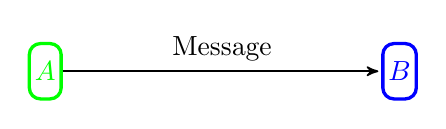
\begin{tikzpicture}[->,>=stealth',shorten >=1pt,auto,node distance=4.5cm, semithick]
  \tikzstyle{every state}=[fill=red,draw=none,text=white]
  \node[state, green]              (A)      {$A$};
  \node[state, blue ,right of=A]   (B)      {$B$};
  \draw (A)            edge[above]          node{Message}   (B);
\end{tikzpicture}

      $A$ is green, i.e in state $A$ the client has agency.
      Therefore the client sends a message to the server and
      both client and server transition to state $B$.
      As $B$ is blue the agency also changes from client to server.

\begin{tikzpicture}[->,>=stealth',shorten >=1pt,auto,node distance=4.5cm, semithick]
  \tikzstyle{every state}=[fill=red,draw=none,text=white]
  \node[state, blue]               (C)      {$C$};
  \node[state, blue ,right of=A]   (D)      {$D$};
  \draw (A)            edge[above]               node{Message}   (B);
\end{tikzpicture}

      $C$ is blue, i.e in state $C$ the server has agency.
      Therefore the server sends a message to the client and
      both client and server transition to state $D$.
      As $D$ is also blue the agency remains at the server.

\item[Client and server implementation]
  The state machine describes which messages are sent and received and in which order.
  This is the external view of the protocol that every compatible implementation MUST follow.
  In addition to the external view of the protocol, this part of the specification describes
  how the client and server actually process the transmitted messages,
  i.e. how the client and server update their internal mutable state
  upon the exchange of messages.

  Strictly speaking, the representation of the node-local mutable state
  and the updates to the node-local state are implementation details that are
  not part of the communication protocol between the nodes,  and will
  depend on an application that is built on top of the network service
  (wallet, core node, explorer, etc.).
  The corresponding sections were added to clarify the mode of operation of the
  mini protocols.

\end{description}
\section{Overview of all implemented Mini Protocols}

\newcommand{\miniEntry}[4]{
  \begin{framed}
      \noindent\textbf{#1}\hfill  Section \ref{#2}
      \newline {#3}
      \newline {\small\texttt{#4}}
  \end{framed}
}

\miniEntry
    {Ping Pong Protocol}
    {ping-pong-protocol}
    {A simple ping-pong protocol for testing.}
    {typed-protocols/src/Network/TypedProtocol/PingPong/Type.hs}

\miniEntry
    {Request Response Protocol}
    {request-response-protocol}
    {A ping pong like protocol which allows to exchanges data.}
    {typed-protocols/src/Network/TypedProtocol/ReqResp/Type.hs}

\miniEntry
    {Chain Synchronisation Protocol}
    {chain-sync-protocol}
    {The protocol by which a downstream chain consumer follows an upstream chain producer.}
    {ouroboros-network/src/Ouroboros/Network/Protocol/ChainSync/Type.hs}

\miniEntry
    {Block Fetch Protocol}
    {block-fetch-protocol}
    {The block fetching mechanism enables a node to download ranges of blocks.}
    {ouroboros-network/src/Ouroboros/Network/Protocol/BlockFetch/Type.hs}

\miniEntry
    {Local Transaction Submission Mini Protocol}
    {local-tx-submission-protocol}
    {Transmitting Transactions from a wallet to a local node.}
    {src/Ouroboros/Network/Protocol/LocalTxSubmission/Type.hs}

\miniEntry
    {Node-to-Node Transaction Submission Protocol}
    {tx-submission-protocol}
    {A Protocol for transmitting transaction between core nodes.}
    {ouroboros-network/src/Ouroboros/Network/Protocol/TxSubmission/Type.hs}

\miniEntry
    {Handshake Mini Protocol}
    {handshake-protocol}
    {This protocol is used for version negotiation.}
    {src/Ouroboros/Network/Protocol/Handshake/Type.hs}

\section{Ping-Pong Protocol}
\label{ping-pong-protocol}
\hsref{typed-protocols/src/Network/TypedProtocol/PingPong/Type.hs}
\newcommand{\Ping}{\msg{Ping}}
\newcommand{\Pong}{\msg{Pong}}

\subsection{Description}
A client can use the Ping-Pong protocol to check that the server is responsive.
The Ping-Pong protocol is very simple because the messages do not carry any data and
because the Ping-Pong client and the Ping-Pong server do not access the internal state of the node.

\subsection{State Machine}

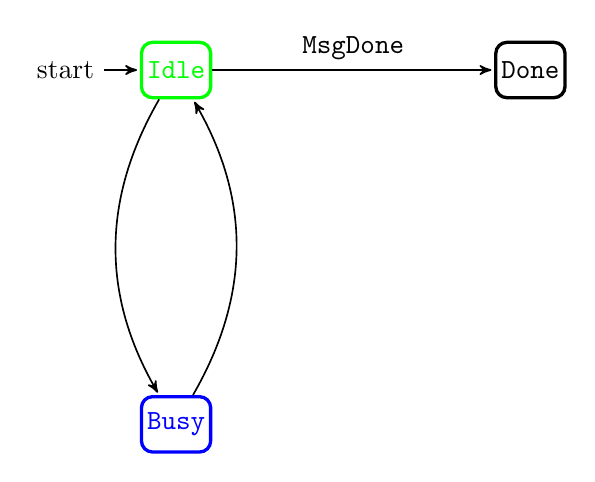
\begin{tikzpicture}[->,>=stealth',shorten >=1pt,auto,node distance=4.5cm, semithick]
  \tikzstyle{every state}=[fill=red,draw=none,text=white]
  \node[state, green, initial]                            (Idle)      {\Idle};
  \node[state, right of=Idle]                             (Done)      {\Done};
  \node[state, blue, below of=Idle]                       (Busy)      {\Busy};

  \draw (Idle)         edge[above]               node{\MsgDone}                  (Done);
  \draw (Idle)         edge[left, bend right]    node{\Ping}                     (Busy);
  \draw (Busy)         edge[right, bend right]   node{\Pong}                     (Idle);
\end{tikzpicture}

\begin{figure}[ht]
\begin{tabular}{|l|l|} \hline
\multicolumn{2}{|c|}{Agency} \\ \hline
  Client has Agency & \Idle \\  \hline
  Server has Agency & \Busy \\  \hline
\end{tabular}
\end{figure}

The protocol uses the following messages.
The messages of the Ping-Pong protocol do not carry any data.
\begin{description}
\item [\Ping]
      The client sends a Ping request to the server.
\item [\Pong]
      The server replies to a Ping with a Pong.
\item [\MsgDone]
      Terminate the protocol.
\end{description}

\begin{tabular}{|l|l|l|}
  \hline
  \multicolumn{3}{|c|}{Transition table} \\ \hline
  from state   & message            & to state    \\ \hline\hline
  \Idle        & \Ping              & \Busy   \\ \hline
  \Busy        & \Pong              & \Idle   \\ \hline
  \Idle        & \MsgDone           & \Done       \\ \hline
\end{tabular}

\section{Request Response Protocol}
\label{request-response-protocol}
\renewcommand{\Idle}{\state{Idle}}
\renewcommand{\Busy}{\state{Busy}}
\renewcommand{\Done}{\state{Done}}
\newcommand{\Request}{\msg{Request}}
\newcommand{\Response}{\msg{Response}}

\subsection{Description}
The request response protocol is polymorphic in the request and response data that is being transmitted.
This means that there are different possible applications of this protocol and the
application of the protocol determines the types of the requests and responses.

\subsection{State machine}
\hsref{ouroboros-network/src/Ouroboros/Network/Protocol/ReqResp/Type.hs}

\begin{tabular}{|l|l|}
  \hline
  \multicolumn{2}{|c|}{Agency} \\ \hline
  Client has Agency & \Idle \\  \hline
  Server has Agency & \Busy \\ \hline
\end{tabular}
{\vskip 10pt}
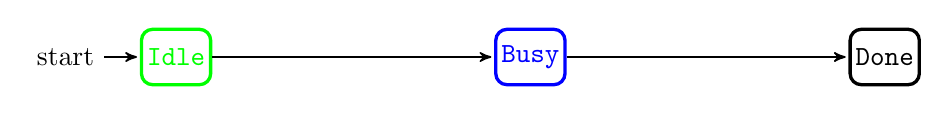
\begin{tikzpicture}[->,>=stealth',shorten >=1pt,auto,node distance=4.5cm, semithick]
  \tikzstyle{every state}=[fill=red,draw=none,text=white]
  \node[state, green, initial]                                   (Idle)      {\Idle};
  \node[state, blue, right of=Idle]                              (Busy)      {\Busy};
  \node[state, right of=Busy]                                    (Done)      {\Done};

  \draw (Idle)         edge[]      node{\Request}           (Busy);
  \draw (Busy)         edge[]      node{\Response}          (Done);
\end{tikzpicture}
{\vskip 10pt}
The protocol uses the following messages.
\begin{description}
\item [\Request{} $(request)$]
      The client sends a request to the server.
\item [\Response{} $(response)$]
      The server replies with a response.
\end{description}

\begin{tabular}{|l|l|l|l|} \hline
\multicolumn{4}{|c|}{Transition table} \\ \hline
  from         & message            & parameters             & to       \\ \hline\hline
  \Idle        & \Request           & $request$              & \Busy     \\ \hline
  \Busy        & \Response          & $response$             & \Done     \\ \hline
\end{tabular}

\section{Chain Synchronisation Protocol}
\label{chain-sync-protocol}
\hsref{ouroboros-network/src/Ouroboros/Network/Protocol/ChainSync/Type.hs}
\newcommand{\CanAwait}{\state{CanAwait}}
\newcommand{\MustReply}{\state{MustReply}}
\newcommand{\Intersect}{\state{Intersect}}
\newcommand{\RequestNext}{\msg{RequestNext}}
\newcommand{\AwaitReply}{\msg{AwaitReply}}
\newcommand{\RollForward}{\msg{RollForward}}
\newcommand{\RollBackward}{\msg{RollBackward}}
\newcommand{\FindIntersect}{\msg{FindIntersect}}
\newcommand{\IntersectFound}{\msg{IntersectFound}}
\newcommand{\IntersectNotFound}{\msg{IntersectNotFound}}

\subsection{Description}
The chain synchronisation protocol is used by a block chain consumer
to replicate the producer's block chain locally.
A node communicates with several upstream and downstream nodes
and runs an independent client instance and a independent server instance for every
other node it communicates with.
(See Figure~\ref{node-diagram-concurrency}.)

The chain synchronisation protocol is polymorphic.
The (full)-node to client protocol uses an instance of the chain synchronisation protocol
that transfers full blocks, while the node-to-node instance only transfers block headers.
In the node-to-node case, the block fetch protocol (Section \ref{block-fetch-protocol})
is used to transfer full blocks.

\subsection{State Machine}

\begin{tabular}{|l|l|}
  \hline
  \multicolumn{2}{|c|}{Agency} \\ \hline
  Client has Agency & \Idle \\  \hline
  Server has Agency & \CanAwait, \MustReply, \Intersect \\ \hline
\end{tabular}

\begin{figure}[ht]
\begin{tikzpicture}[->,>=stealth',shorten >=1pt,auto,node distance=4.5cm, semithick]
  \tikzstyle{every state}=[fill=red,draw=none,text=white]
  \node[state, green, initial]                            (Idle)      {\Idle};
  \node[state, right of=Idle]                             (Done)      {\Done};
  \node[state, blue, below left of=Idle]                  (CanAwait)  {\CanAwait};
  \node[state, blue, right of=CanAwait]                   (MustReply) {\MustReply};
  \node[state, blue, above of=Idle]                       (Intersect) {\Intersect};

  \draw (Idle)         edge[left, bend right]      node{\RequestNext}           (CanAwait);
  \draw (CanAwait)     edge[below, bend right]     node{\AwaitReply}            (MustReply);
  \draw (CanAwait)     edge[above,bend right=45]     node{\RollForward}           (Idle);
  \draw (MustReply)    edge[right,bend right=45]     node{\RollForward}           (Idle);
  \draw (CanAwait)     edge[above,bend right=80]     node{\RollBackward}          (Idle);
  \draw (MustReply)    edge[right,bend right=80]     node{\RollBackward}          (Idle);
  \draw (Idle)         edge[right, bend right]    node{\FindIntersect}         (Intersect);
  \draw (Intersect)    edge[above, bend right=45]    node[below = 4mm]{\IntersectFound}     (Idle);
  \draw (Intersect)    edge[above, bend right=80]    node[above = 4mm]{\IntersectNotFound}  (Idle);
  \draw (Idle)         edge[above]                node{\MsgDone}                  (Done);
\end{tikzpicture}
\caption{State machine of the chain sync protocol.}
\label{chain-sync-automata}
\end{figure}

The protocol uses the following messages:
\begin{description}
\item [\RequestNext]
      Request the next update from the producer.
\item [\AwaitReply]
      Acknowledge the request but require the consumer to wait for the next update.
      This means that the consumer is synced with the producer, and
      the producer is waiting for its own chain state to change.
\item [\RollForward{} {\boldmath $(header, tip)$}]
      Tell the consumer to extend their chain with the given $header$.
      The message also tells the consumer about the $tip$ of the producers chain.
\item [\RollBackward{} {\boldmath $(point_{old}, tip$}]
      Tell the consumer to roll back to a given $point_{old}$ on their chain.
      The message also tells the consumer about the current  $tip$ of the chain the producer is following.
\item [\FindIntersect{} {\boldmath $\langle point_{head} \rangle $}]
      Ask the producer to try to find an improved intersection point between
      the consumer and producer's chains.
      The consumer sends a sequence {\boldmath $\langle point \rangle $}
      and it is up to the producer
      to find the first intersection point on its chain and send it back to the consumer.
\item [\IntersectFound{} {\boldmath $(point_{intersect} ,tip)$}]
      The producer replies with the first point of the request that is on his current chain.
      The consumer can decide whether to send more points.
      The message also tells the consumer about the $tip$ of the producer.
\item [\IntersectNotFound{} {\boldmath $(tip)$}]
      The reply to the consumer that no intersection was found: none of the
      points the consumer supplied are on the producer chain.
      The message only contains the $tip$ of the producer chain.
\item [\MsgDone]
      Terminate the protocol.
\end{description}

\begin{tabular}{|l|l|l|l|}
  \hline
  \multicolumn{4}{|c|}{Transition table} \\ \hline
  from state & message             & parameters                          & to state    \\ \hline\hline
  \Idle      & \RequestNext        &                                     & \CanAwait   \\ \hline
  \Idle      & \FindIntersect      & $\langle point\rangle$              & \Intersect  \\ \hline
  \Idle      & \MsgDone            &                                     & \Done       \\ \hline
  \CanAwait  & \AwaitReply         &                                     & \MustReply  \\ \hline
  \CanAwait  & \RollForward        & $header$, $tip$                     & \Idle       \\ \hline
  \CanAwait  & \RollBackward       & $header_{old}$, $tip$                & \Idle       \\ \hline
  \MustReply & \RollForward        & $header$, $tip$                     & \Idle       \\ \hline
  \MustReply & \RollBackward       & $point_{old}$, $tip$                 & \Idle       \\ \hline
  \Intersect & \IntersectFound     & $point_{intersect}$, $tip$            & \Idle       \\ \hline
  \Intersect & \IntersectNotFound  & $tip$                               & \Idle       \\ \hline

\end{tabular}

\newcommand{\readpointer}{\emph{read-pointer}}
\subsection{Implementation of the Chain Producer}
\hide{The trade-offs between the robustness and efficiency of possible chain-sync protocols are
discussed in Section~\ref{chain-sync-discussion}.
}
This section describes a state-full implementation of a chain producer that is suitable for a setting where
the producer cannot trust the chain consumer.
An important requirement in this setting
is that a chain consumer must never be able to cause excessive resource use on the producer side.
The presented implementation meets this requirement.
It uses a constant amount of memory to store the state that the producer maintains
per chain consumer.  This protocol is only used to reproduce the producer
chain locally by consumer.  By running many instances of this protocol against
different peers, a node can reproduce chains in the network and
do chain selection which by design is not part of this protocol.
Note, that when we refer to the consumer's chain in this section, we mean
the chain that is reproduced by the consumer with the instance of
the chain-sync protocol under consideration and not the result of the chain selection algorithm.

We call the state which the producer maintains about the consumer the \readpointer{}.
The \readpointer{} basically tracks what the producer knows about the head of
the consumer's chain without storing it locally.
It points to a block on the current chain of the chain producer.
The \readpointer{}s are part of the shared state of the node (Figure~\ref{node-diagram-concurrency}) and
\readpointer{}s are concurrently updated by the thread that runs the chain-sync mini-protocol and the
chain tracking logic of the node itself.

We first describe how the mini-protocol updates a \readpointer{} and later address what happens in case
of a fork.
\subparagraph{Initializing the \readpointer{}.}
The chain producer assumes that a consumer, which has just connected,
only knows the genesis block and initialises the \readpointer{} of that consumer
with a pointer to the genesis block on its chain.

\subparagraph{Downloading a chain of blocks}
A typical situation is when the consumer follows the chain of the producer but is not yet at the head of the
chain (this also covers a consumer booting from genesis).
In this case, the protocol follows a simple, consumer-driven, request-response pattern.
The consumer sends \RequestNext{} messages to ask for the next block.
If the \readpointer{} is not yet at the head of the chain,
the producer replies with a \RollForward{} and advances the \readpointer{} to
the next block (optimistically assuming that the client will update its chain
accordingly).
The \RollForward{} message contains the next block and also the head-point of the producer.
The protocol follows this pattern until the \readpointer{} reaches the end of its chain.

\begin{figure}[ht]
\pgfdeclareimage[height=7cm]{read-pointer-consumer-driver}{figure/read-pointer-consumer-driven.pdf}
\begin{center}
\pgfuseimage{read-pointer-consumer-driver}
\end{center}
\caption{Consumer driven block download.}
\label{read-pointer-consumer-driver}
\end{figure}

\subparagraph{Producer driven updates}
If the \readpointer{} points to the end of the chain and the producer receives
a \RequestNext{}
the consumers chain is already up to date.
The producer informs the consumer with an \AwaitReply{} that no new data is available.
After receiving a \AwaitReply, the consumer just waits for a new message and the producer keeps agency.
The \AwaitReply{} switches from a consumer driven phase to a producer driven phase.

The producer waits until new data becomes available.
When a new block is available, the producer will
send a \RollForward{} message and give agency back to the consumer.
The producer can also get unblocked when its node switches to a new chain fork.

\subparagraph{Producer switches to a new fork}
The node of the chain producer can switch to a new fork at any time, independent of the
state machine.
A chain switch can cause an update of the \readpointer{},
which is part of the mutable state that is shared between the thread that runs
the chain sync protocol and the thread that implements the chain following logic of the node.
There are two cases:

1) If the \readpointer{} points to a block that is on the common prefix of the new
fork and the old fork, no update of the \readpointer{} is needed.

2) If the \readpointer{} points to a block that is no longer part of the chain that is followed by the node,
the \readpointer{} is set to the last block that is common between the new and the old chain.
The node also sets a flag that signals the chain-sync thread to send a \RollBackward{} instead
of a \RollForward.
Finally the producer thread must unblock if it is in the \MustReply{} state.

\begin{figure}[ht]
\pgfdeclareimage[height=5cm]{read-pointer-rollback}{figure/read-pointer-rollback.pdf}
\begin{center}
\pgfuseimage{read-pointer-rollback}
\end{center}
\caption{\readpointer{} update for a fork switch in case of a rollback.}
\label{read-pointer-rollback}
\end{figure}

Figure~\ref{read-pointer-rollback} illustrates a fork switch that requires an update of the \readpointer{}
for one of the chain consumers, i.e. an example for case 2.
Before the switch, the \readpointer{} of the consumer points to block $0x660f$.
The producer switches to a new chain with the head of the chain at block $0xcdf0$.
The node must update the \readpointer{} to block $0xfa40$ and the next message to the consumer
will be a \RollBackward.

Note, that a node typically communicates with several consumers. For each consumer it runs an independent
version of the chain-sync-protocol state machine in an independent thread and with its own \readpointer{}.
Each of those \readpointer{}s has to be updated independently and for each consumer
either case 1) or case 2) can apply.

\subparagraph{Consumer starts with an arbitrary fork}
Typically, the consumer already knows some fork of the block chain when it
starts to track the producer.
The protocol provides an efficient method to search for the longest common prefix (here called intersection)
between the fork of the producer and the fork that is known to the consumer.

To do so, the consumer sends a \FindIntersect{} message with a list of chain
points on the chain known to the consumer.
If the producer does not know any of the points it replies with \IntersectNotFound.
Otherwise it replies with \IntersectFound{} and the best (i.e. the newest) of the points that it knows
and also updates the \readpointer{} accordingly.
For efficiency, the consumer should use a binary search scheme to search for the longest common
prefix.

It is advised that the consumer always starts with \FindIntersect{} in a fresh connection
and it is free to use \FindIntersect{} at any time later as seems beneficial.
If the consumer does not know anything about the producer's chain,
it can start the search with the following list of points:
$\langle point(b), point(b-1), point(b-2), point(b-4), point (b-8),\ldots \rangle$
where $point(b-i)$ is the point of the $i$th predecessor of block $b$ and
$b$ is the head of the consumer fork.
Maximum depth of a fork in Ouroboros is bounded and the intersection will always be found with a small number of
iterations of this algorithm.

\subsection{Implementation of the Chain Consumer}
In principle, the chain consumer has to guard against a malicious chain producer
as much as the other way around.
However, two aspects of the protocol play in favour of the consumer here.
\begin{itemize}
  \item The protocol is basically consumer driven, i.e. the producer has no way to send unsolicited
data to the consumer (within the protocol).
  \item The consumer can verify the response data itself.
\end{itemize}
Here are some cases to consider:
\begin{description}
\item[\FindIntersect~Phase]
  The consumer and the producer play a number guessing game, so the consumer can easily detect
  inconsistent behaviour.
\item[The producer replies with a \RollForward] The consumer can verify the block itself
  with the help of the ledger layer.
  (The consumer may need to download the block first, if the protocol only sends block headers.)
\item[The producer replies with a \RollBackward] The consumer tracks several producers, so
  if the producer sends false \RollBackward{} messages the consumer's node
  will, at some point, just switch to a longer chain fork.
\item[The Producer is just passive/slow] The consumer's node will switch to
  a longer chain coming from another producer via another instance of
    chain-sync protocol.
\end{description}

\section{Block Fetch Protocol}
\label{block-fetch-protocol}

\hsref{ouroboros-network/src/Ouroboros/Network/Protocol/BlockFetch/Type.hs}
\renewcommand{\Idle}{\state{Idle}}
\renewcommand{\Busy}{\state{Busy}}
\newcommand{\Streaming}{\state{Streaming}}
\renewcommand{\Done}{\state{Done}}
\newcommand{\RequestRange}{\msg{RequestRange}}
\newcommand{\StartBatch}{\msg{StartBatch}}
\newcommand{\NoBlocks}{\msg{NoBlocks}}
\newcommand{\Block}{\msg{Block}}
\newcommand{\BatchDone}{\msg{BatchDone}}
\newcommand{\ClientDone}{\msg{ClientDone}}

\subsection{Description}

The block fetching mechanism enables a node to download a range of blocks.

\subsection{State machine}

\begin{tabular}{|l|l|}
  \hline
  \multicolumn{2}{|c|}{Agency} \\ \hline
  Client has Agency & \Idle            \\  \hline
  Server has Agency & \Busy, \Streaming \\ \hline
\end{tabular}

\begin{tikzpicture}[->,>=stealth',shorten >=1pt,auto,node distance=4.5cm, semithick]
  \tikzstyle{every state}=[fill=red,draw=none,text=white]
  \node[state, green, initial]                            (Idle)      {\Idle};
  \node[state, right of=Idle]                             (Done)      {\Done};
  \node[state, blue, below left of=Idle]                  (Busy)      {\Busy};
  \node[state, blue, right of=CanAwait]                   (Streaming) {\Streaming};

  \draw (Idle)         edge[above]                node{\ClientDone}                  (Done);
  \draw (Idle)         edge[left,bend right]      node{\RequestRange}                (Busy);
  \draw (Busy)         edge[above,bend right]     node{\NoBlocks}                    (Idle);
  \draw (Busy)         edge[below]                node{\StartBatch}                  (Streaming);
  \draw (Streaming)    edge[loop right]           node{\Block}                       (Streaming);
  \draw (Streaming)    edge[right]                node{\BatchDone}                   (Idle);
\end{tikzpicture}

\begin{description}
\item [\RequestRange{} {\boldmath $(range)$}]
  The client requests a {\boldmath $range$} of blocks from the server.
\item [\NoBlocks]
  The server tells the client that it does not have blocks.
\item [\StartBatch]
  The server starts block streaming.
\item [\Block{} {\boldmath $(body)$}]
  Stream a single block's body.
\item [\BatchDone]
  The server ends block streaming.
\item [\ClientDone]
  The client terminates the protocol.
\end{description}

Transition table:

\begin{tabular}{|l|l|l|l|}
  \hline
  \multicolumn{4}{|c|}{Transition table} \\ \hline
  from state   & message             & parameters             & to state    \\ \hline\hline
  \Idle        & \ClientDone         &                        & \Done       \\ \hline
  \Idle        & \RequestRange       & $range$                & \Busy       \\ \hline
  \Busy        & \NoBlocks           &                        & \Idle       \\ \hline
  \Busy        & \StartBatch         &                        & \Streaming  \\ \hline
  \Streaming   & \Block              & $body$                 & \Streaming  \\ \hline
  \Streaming   & \BatchDone          &                        & \Idle       \\ \hline
\end{tabular}

\section{Local Transaction Submission Mini Protocol}
\hsref{src/Ouroboros/Network/Protocol/LocalTxSubmission/Type.hs}
\label{local-tx-submission-protocol}
\subsection{Description}
The local transaction submission mini protocol is used by local clients,
for example wallets or CLI tools, to submit transactions to a local node.
The protocol is {\bf not} used to forward transactions from one core node to an other.
The protocol for the transfer of transactions between full nodes
is described in Section \ref{tx-submission-protocol}.

The protocol follows a simple request-response pattern:
\begin{enumerate}
\item The client sends a request with a single transaction.
\item The Server either accepts the transaction (returning a confirmation) or rejects it (returning the
  reason).
\end{enumerate}
Note, that the local transaction submission protocol is a push based protocol where the client
creates a workload for the server.
This is acceptable because is protocol is only for use between a node and local client.
\newcommand{\SubmitTx}{\trans{SubmitTx}}
\newcommand{\AcceptTx}{\trans{AcceptTx}}
\newcommand{\RejectTx}{\trans{RejectTx}}
\subsection{State machine}

\begin{tabular}{|l|l|}
  \hline
  \multicolumn{2}{|c|}{Agency} \\ \hline
  Client has Agency & \Idle \\ \hline
  Server has Agency & \Busy \\  \hline
\end{tabular}

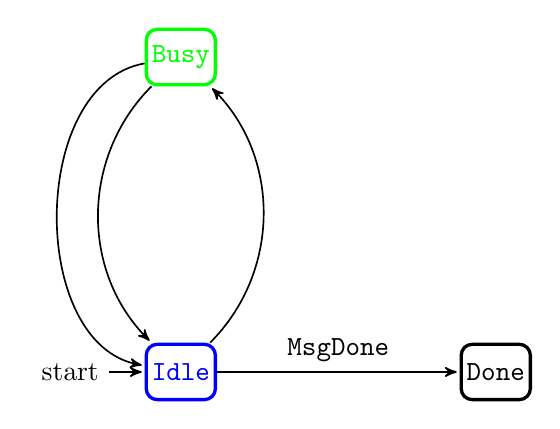
\begin{tikzpicture}[->,>=stealth',shorten >=1pt,auto,node distance=4cm, semithick]
  \tikzstyle{every state}=[fill=red,draw=none,text=white]
  \node[state, blue, initial]                                     (Idle)       {\Idle};
  \node[state, right of=Idle]                                     (Done)       {\Done};
  \node[state, green, above of=Idle]                              (Busy)     {\Busy};

  \draw (Idle)         edge[]                          node{\MsgDone}           (Done);
  \draw (Idle)         edge[right, bend right=45]      node{\SubmitTx}          (Busy);
  \draw (Busy)         edge[left, bend right=45]       node[below = 3mm]{\AcceptTx}          (Idle);
  \draw (Busy)         edge[left, bend right=80]       node[above = 3mm]{\RejectTx}          (Idle);
\end{tikzpicture}

Messages of the protocol:
\begin{description}
\item [\SubmitTx{} {\boldmath $(t)$}]
      The client submits a transaction.
\item [\AcceptTx]
      The server accepts the transaction.
\item [\RejectTx{} {\boldmath $(reason)$}]
      The server rejects the transactions and replies with the $reason$.
\item [\MsgDone]
      The client terminates the mini protocol.
\end{description}

\section{Node-to-Node Transaction Submission Protocol}
\hsref{ouroboros-network/src/Ouroboros/Network/Protocol/TxSubmission/Type.hs}
\label{tx-submission-protocol}
\newcommand{\TxIdsBlocking}   {\state{TxIdsBlocking}}
\newcommand{\TxIdsNonBlocking}{\state{TxIdsNonBlocking}}
\newcommand{\Txs}             {\state{Txs}}
\newcommand{\RequestTxIdsNB}  {\trans{RequestTxIdsNonBlocking}}
\newcommand{\RequestTxIdsB}   {\trans{RequestTxIdsBlocking}}
\newcommand{\ReplyTxIds}      {\trans{ReplyTxIds}}
\newcommand{\RequestTxs}      {\trans{RequestTxs}}
\newcommand{\ReplyTxs}        {\trans{ReplyTxs}}

\subsection{Description}
The node-to-node transaction submission protocol is used to transfer transactions between full nodes.
The protocol follows a pull-based strategy where the initiator asks for new transactions and the responder
replies with the transactions.
It is suitable for a trustless setting where both sides need to guard against resource consumption attacks from
the other side.
The local transaction submission protocol, which is used when the server trusts a local client,
is described in Section \ref{local-tx-submission-protocol}.
The implementation of the node-to-node transaction mini protocol is based on a generic mini protocol framework
(the same as for all other mini protocols).
For technical reasons however the roles of the initiator and the responder are reversed with respect to
the way the other mini protocols are implemented in the frame work.
In other words: The Server is the initiator and ask for new transactions
and the Client is the responder and replies with the transactions.
\subsection{State machine}

\begin{tabular}{|l|l|}
  \hline
  \multicolumn{2}{|c|}{Agency} \\ \hline
  Server has Agency & \Idle \\  \hline
  Client has Agency & \TxIdsBlocking, \TxIdsNonBlocking, \Txs \\ \hline
\end{tabular}

\begin{figure}[h]
\begin{tikzpicture}[->,>=stealth',shorten >=1pt,auto,node distance=4.5cm, semithick]
  \tikzstyle{every state}=[fill=red,draw=none,text=white]
  \node[state, blue, initial](A) at ( 0,  0) {\Idle};
  \node[state]               (B) at ( 8, -4) {\Done};
  \node[state, green]        (C) at ( 4, -4) {\TxIdsBlocking};
  \node[state, green]        (D) at (-4, -4) {\TxIdsNonBlocking};
  \node[state, green]        (E) at ( 0,  4) {\Txs};
  \draw (C)  edge[above]                    node[below]{\MsgDone}                                 (B);
  \draw (A)  edge[left, bend left=45]       node[fill = white, anchor = center]{\RequestTxIdsB}   (C);
  \draw (C)  edge[right, bend left=15]      node[fill = white, anchor = center, above = 2pt]{\ReplyTxIds}     (A);
  \draw (A)  edge[right, bend left=15]      node[fill = white, anchor = center, below = 2pt]{\RequestTxIdsNB} (D);
  \draw (D)  edge[right, bend left=45]      node[fill = white, anchor = center]{\ReplyTxIds}      (A);
  \draw (A)  edge[left, bend right=45]      node[fill = white, anchor = center]{\RequestTxs}      (E);
  \draw (E)  edge[right,bend right=45]      node[fill = white, anchor = center]{\ReplyTxs}        (A);
\end{tikzpicture}
\caption{State machine of the transaction submission protocol.}
\label{tx-submission-automata}
\end{figure}
Messages of the protocol:
\begin{description}
\item [\RequestTxIdsB{} {\boldmath $(ack,req)$}]
      The server asks for new transaction ids and acknowledges old ids.
      The client will block until new transactions are available.
\item [\RequestTxIdsNB{} {\boldmath $(ack,req)$}]
      The server asks for new transaction ids and acknowledges old ids.
      The client immediately replies (possible with an empty list).
\item [\ReplyTxIds{} {\boldmath ($\langle (id, size) \rangle$) }]
      The client replies with a list of available transactions.
      The list contains pairs of transactions ids and the corresponding size of the transaction in bytes.
      In the blocking case the reply is guaranteed to contain at least one transaction.
      In the non-blocking case, the reply may contain an empty list.
\item [\RequestTxs{} {\boldmath ($\langle ids \rangle$)}]
      The server requests transactions by sending a list of transaction-ids.
\item [\ReplyTxs{} {\boldmath ($\langle txs \rangle$})]
      The client replies with a list transaction.
\item [\MsgDone]
      The client terminates the mini protocol.
\end{description}

\begin{tabular}{|l|l|l|l|}
  \hline
  \multicolumn{4}{|c|}{Transition table} \\ \hline
  from state        & message             & parameters                    & to state          \\ \hline\hline
  \Idle             & \RequestTxIdsB      & $ack$,$req$                   & \TxIdsBlocking    \\ \hline
  \TxIdsBlocking    & \ReplyTxIds         & $\langle (id, size) \rangle$  & \Idle             \\ \hline
  \Idle             & \RequestTxIdsNB     & $ack$,$req$                   & \TxIdsNonBlocking \\ \hline
  \TxIdsNonBlocking & \ReplyTxIds         & $\langle (id, size) \rangle$  & \Idle             \\ \hline
  \Idle             & \RequestTxs         & $\langle ids \rangle$         & \Txs              \\ \hline
  \Txs              & \ReplyTxs           & $\langle txs \rangle$         & \Idle             \\ \hline
  \RequestTxIdsB    & \MsgDone            &                               & \Done             \\ \hline
\end{tabular}

\subsection{Client and Server Implementation}
The protocol has two design goals: It must diffuse transactions with high efficiency
and, at the same time, it must rule out
asymmetric resource attacks from the transaction consumer against the transaction provider.

The protocol is based on two pull-based operations.
The transaction consumer can ask for a number of transaction ids and it can use these
transaction ids to request a batch of transactions.
The transaction consumer has flexibility in the number of transaction ids it requests,
whether to actually download the transaction body of a given id
and flexibility in how it batches the download of transactions.
The transaction consumer can also switch between requesting transaction ids and downloading
transaction bodies at any time.
It must however observe several constraints that are necessary for a memory efficient implementation
of the transaction provider.

Conceptually, the provider maintains a limited size FIFO of outstanding transactions per consumer.
(The actual implementation can of course use the data structure that works best).
The maximum FIFO size is a protocol parameter.
The protocol guarantees that, at any time, the consumer and producer agree on the current size of
that FIFO and on the outstanding transaction ids.
The consumer can use a variety of heuristics for requesting transaction ids and transactions.
One possible implementation for a consumer is to maintain a FIFO which mirrors the producers FIFO
but only contains the transaction ids (and the size of the transaction) and not the full transactions.

After the consumer requests new transaction ids, the provider replies with a list of transaction ids and
puts these transactions in its FIFO.
As part of a request a consumer also acknowledges the number of old transactions,
which are removed from the FIFO at the same time.
The provider checks that the size of the FIFO, i.e. the number of outstanding transactions,
never exceeds the protocol limit and aborts the connection if a request violates the limits.
The consumer can request any batch of transactions from the current FIFO in any order.
Note however, that the reply will omit any transactions that have become invalid in the meantime.
(More precisely the server will omit invalid transactions from the reply but they will still be counted in the FIFO
size and they still require a acknowledgement from the consumer).

The protocol supports blocking and non-blocking requests for new transactions ids.
If the FIFO is empty the consumer must use a blocking request
otherwise a non-blocking request.
The producer must reply immediately (i.e. within a small timeout) to a non-blocking request.
It replies with not more then the requested number of ids (possible with an empty list).
A blocking request on the other side, waits until at least one transaction is available.

\section{Handshake Mini Protocol}
\hsref{src/Ouroboros/Network/Protocol/Handshake/Type.hs}
\label{handshake-protocol}
\newcommand{\StPropose}{\state{StPropose}}
\newcommand{\StConfirmAny}{\state{StConfirm peerRole}}
\newcommand{\StConfirmAsServer}{\state{StConfirm AsServer}}
\newcommand{\StConfirmAsClient}{\state{StConfirm AsClient}}
\newcommand{\MsgProposeVersions}{\msg{MsgProposeVersions}}
\newcommand{\MsgProposeVersionsX}{\msg{MsgProposeVersions'}}
\newcommand{\MsgAcceptVersion}{\msg{MsgAcceptVersion}}
\newcommand{\MsgRefuse}{\msg{MsgRefuse}}

\newcommand{\VersionMismatch}{\msg{VersionMismatch}}
\newcommand{\HandshakeDecodeError}{\msg{HandshakeDecodeError}}
\newcommand{\Refused}{\msg{Refused}}

\subsection{Description}
The handshake mini protocol is used to negotiate the protocol version
and the protocol parameters that are used by the client and the server.
It is run exactly once when a new connection is initialised
and consists of a single request from the client and a single reply from the server.
Section \ref{peer-setup-section} explains the live cycle of a connection and the role of
the handshake mini protocol in more detail.

The handshake mini protocol is a generic protocol that can negotiate any kind protocol parameters.
It only assumes that protocol parameters can be encoded to, and decoded from, CBOR terms.
A node, that runs the handshake protocol, must instantiate it with the set of
supported protocol versions and callback functions for handling the protocol parameters.
These callback functions are specific for the supported protocol versions.

The handshake mini protocol can also handle simultantous TCP open.  For that
resason its state machine is more complex than a request reponse protocol.

\subsection{State machine}

\begin{tabular}{|l|l|}
  \hline
  \multicolumn{2}{|c|}{Agency}   \\ \hline
  Client has Agency & \StPropose, \StConfirmAsClient \\ \hline
  Server has Agency & \StConfirmAsServer \\ \hline
\end{tabular}

\begin{tikzpicture}[->,>=stealth',shorten >=1pt,auto,node distance=5cm, semithick]
  \tikzstyle{every state}=[fill=red,draw=none,text=white]
  \node[state, green, initial]   (StPropose)         at (0,  0)  {\StPropose};
  \node[state, blue]             (StConfirmAsServer) at (4,  2)  {\StConfirmAsServer};
  \node[state, green]            (StConfirmAsClient) at (4, -2) {\StConfirmAsClient};
  \node[state, right of=Confirm] (StDone)            at (7,  0)  {\StDone};

  \draw (StPropose) edge[] node{\MsgProposeVersions} (StConfirmAsServer);
  \draw[->] (StConfirmAsServer.10)  to [out=5, in=160]  node[above right]{\MsgAcceptVersion} (StDone.west);
  \draw[->] (StConfirmAsServer.350) to [out=-5, in=170] node[below left]{\MsgRefuse} (StDone.west);
  \draw[->] (StConfirmAsServer)     -- node[fill=white, right=-60pt]{\MsgProposeVersions} (StConfirmAsClient);
  \draw[->] (StConfirmAsClient.10)  to [out=5, in=190]  node[above left]{\MsgAcceptVersion} (StDone.west);
  \draw[->] (StConfirmAsClient.350) to [out=-5, in=200] node[below right]{\MsgRefuse} (StDone.west);
\end{tikzpicture}

Messages of the protocol:
\begin{description}
\item [\MsgProposeVersions{} {\boldmath $(versionTable)$}]
      The client proposes a number of possible versions and protocol parameters.
      In TCP simultanous open the client will receive
      \MsgProposeVersions{} as a reply to \MsgProposeVersions{}.
\item [\MsgAcceptVersion{} {\boldmath $(versionNumber,extraParameters)$}]
      The server accepts $versionNumber$ and returns possible extra protocol parameters.
\item [\MsgRefuse{} {\boldmath $(reason)$}]
      The server refuses the proposed versions.
\end{description}

{\small
\begin{tabular}{|l|l|l|l|} \hline
\multicolumn{4}{|c|}{Transition table} \\ \hline
  from               & message/event         & parameters                        & to \\ \hline\hline
  \StPropose         & \MsgProposeVersions   & $versionTable$                    & \StConfirmAsServer \\ \hline
  \StConfirmAsServer & \MsgProposeVersions   & $versionTable$                    & \StConfirmAsClient \\ \hline
  \StConfirmAny      & \MsgAcceptVersion     & $(versionNumber,extraParameters)$ & \StDone \\ \hline
  \StConfirmAny      & \MsgRefuse            & $reason$                          & \StDone \\ \hline
\end{tabular}
}

\subsection{Client and Server Implementation}
Section~\ref{included-cddl} contains the CDDL-specification of the binary format of the handshake messages.
The version table is encoded as a CBOR table with the version number as key
and the protocol parameters as value.
The handshake protocol requires that the version numbers ( i.e. the keys) in the version table are unique
and appear in ascending order.
(Note, that CDDL is not expressive enough to precisely specify that requirement on the keys of the CBOR
table. Therefor the CDDL-specification uses a table with keys from 1 to 4 as an example.)

In a run of the handshake mini protocol the peers exchange only two messages:
The client requests to connect with a \MsgProposeVersions{} message that contains information about
all protocol versions it wants to support.
The server replies either with an \MsgAcceptVersion{} message containing the negotiated
version number and extra parameters or a \MsgRefuse{} message.
The \MsgRefuse{} message contains one of three alternative refuse reasons:
\VersionMismatch{}, \HandshakeDecodeError{} or just \Refused{}.

When a server receives a \MsgProposeVersions{} message it uses the following algorithm to
compute the response:
\begin{enumerate}
\item
  Compute the intersection of the set of protocol version numbers that the server support
  and the version numbers requested by the client.
\item
  If the intersection is empty:
  Reply with \MsgRefuse(\VersionMismatch) and the list of protocol numbers the server supports.
\item
  Otherwise:
  Select the protocol with the highest version number in the intersection.
\item
  Run the protocol specific decoder on the CBOR term that contains the protocol parameters.
\item
  If the decoder fails:
  Reply with \MsgRefuse(\HandshakeDecodeError), the selected version number and an error message.
\item
  Otherwise: Test the proposed protocol parameters of the selected protocol version
\item
  If the test refuses the parameters:
  Reply with \MsgRefuse(\Refused), the selected version number and an error message.
\item
  Otherwise:
  Encode the extra parameters and
  reply with \MsgAcceptVersion, the selected version number and the extra parameters.
\end{enumerate}
Note, that in step 4), 6) and 8) the handshake protocol uses the callback functions that are specific
for set of protocols that the server supports.
The handshake protocol is designed,
such that a server can always handle requests for protocol versions that it does not support.
The server simply ignores the CBOR terms that represent the protocol parameters of unsupported
version.

The handshake mini protocol runs before the MUX/DEMUX itself is initialised.
Each message is transmitted within a single MUX segment, i.e. with a proper
segment header, but, as the MUX/DEMUX is not yet running the messages must not
be split into multiple segments.  These MUX segments are using a reserved
protocol id $0$ (\texttt{Muxcontrol}).

\section{Pipelining of Mini Protocols}
\label{pipelining}
Protocol pipelining is a technique that improves the performance of some protocols.
The underlying idea is that a client, which wants to perform several requests,
just transmits those requests in sequence without blocking and waiting for the reply from the server.
In the reference implementation, pipelining is used by the clients of all mini protocol except Chain-Sync.
Those mini protocols follow a request-response pattern that is amenable to pipelining such
that pipelining becomes a feature of the client implementation that does not require any
modifications of the server implementation.

As an example, let's consider the Block-Fetch mini protocol.
When a client follows the protocol and sends a sequence of \RequestRange~messages to the server
the data stream from the client to the server will only consist of \RequestRange~messages
(and a final \ClientDone~message) and no other message types.
The server can simply follow the state machine of the protocol and process the messages in turn,
regardless whether the client uses pipelining or not.
The MUX/DEMUX layer (Section~\ref{multiplexing-section}) guarantees
that messages of the same mini protocol are delivered in transmission order,
and therefore the client can determine which response belongs to which request.

The MUX/DEMUX layer also provides a fixed size buffer between the egress of DEMUX and the ingress
of mini protocol thread.
The size of this buffer is a protocol parameter that determines how many messages
a client can send before waiting for a reply from the server (see Section~\ref{mux-flow-control}).
The protocol requires that a client must never cause a overrun of these buffers on a server node.
If a message arrives at the server that would cause the buffer to overrun,
the server treats this case as a protocol violation of the peer
(and closes the connection to the peer).
\hide{
The buffer sizes are listed in Table~\ref{bla} in Section~\ref{blub}.
}

\wip{
  \section{DeltaQ Mini Protocol}

  WIP : Explain DeltaQ measurement back pressure and how we deal with slow
  connection.  See Section % ~\ref{deltaq-discussion}.  The DeltaQ mini
  protocol does not transmit is own messages.  Instead it relies on the time
  stamps that the multiplexing layer (Section~\ref{multiplexing-section}) adds
  to the messages of other mini protocols.
}


\include{mux}
% \include{rest}
\appendix
\include{cddl}
\bibliographystyle{apalike}
\bibliography{references}

\end{document}
